\documentclass[12pt]{article} % use larger type; default would be 10pt

\usepackage[utf8]{inputenc} % set input encoding (not needed with XeLaTeX)

\usepackage{graphicx}

\usepackage{listings}
\usepackage[scaled]{beramono}
\usepackage[T1]{fontenc}

\lstset{basicstyle= \footnotesize\ttfamily, language=Logo, tabsize = 2, showspaces= false, showstringspaces=false, breaklines =true, captionpos=b, frame=trBL}







%%% The "real" document content comes below...

\title{Simulation of the Nomification of Independent Chord Rings}
\author{Andrew Rosen \qquad Brendan Benshoof }
\date{} % Activate to display a given date or no date (if empty),
         % otherwise the current date is printed 

\begin{document}
\maketitle
\newpage
\section{Problem Space}

The most important component of a decentralized peer-to-peer network is the ability of nodes to find the various files and data stored in the network \cite{Chord}.  While such a task is simple in a centralized network, the challenge is monstrous in a decentralized network.  The lookup protocol must be quick:  preferably a $log n$ lookup time.  The protocol must be robust; able to deal with the inherent volatility of decentralized system, with multiple nodes joining and leaving at any given time.  The protocol must also be straightforward to implement.

Hashing protocols such as Kademlia \cite{Kademlia}, popularized due to its implementation in BitTorrent \cite{BitTorrent}, address these challenges with great success.  Our paper examines the implementation of another, older hashing protocol named Chord \cite{Chord} and some of the difficulties surrounding the implementation.
\subsection{Chord}

The Chord protocol \cite{Chord} takes in some key and returns the identity (ID) of the node responsible for that key.  These keys are generated by hashing a value of the node, such as the IP address, or by hashing  the filename of a file.  The hashing process creates a $m$-bit hash identifier\footnote{In our simulation, this hash-id is randomly generated for each node.}, where $2^m$ is the maximum number of nodes in the network.

The nodes are then arranged in a ring from the lowest hash-value to highest.  Chord then takes the hashed files and places each in the node that has the same hashed identifier as it.  If no such node exists, the node with the first identifier that follows this value.  This node responsible for the key $\kappa$ is called the $successor$ of $\kappa$, or $successor(\kappa)$.  Since we are dealing with a circle, this assignment is done in module $2^m$ space.  For example, if there were some portion of the network with nodes 20, 25, and 27, node 25 could be responsible for the files with the keys (21,22,23,24,25). If node 25 were to decide to leave the network, it would inform node 27, who would then be responsible for all the keys node 25 was covering. An example Chord network is drawn in in Figure \ref{chordreal}.


\begin{figure}
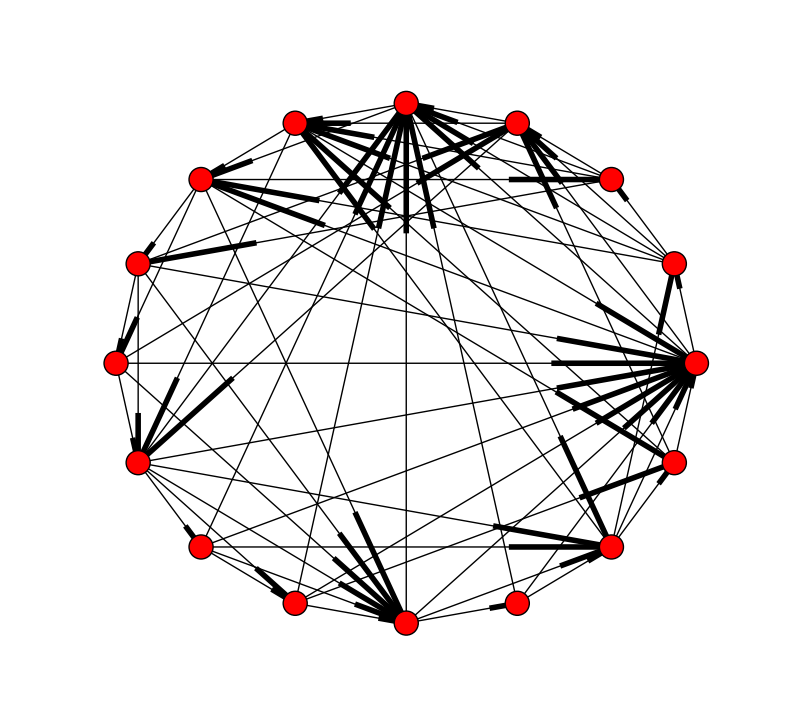
\includegraphics[width=\linewidth]{chordreal}
\caption{An example size 16 network produced by the simulation.  The lines edges are incoming edges.  Note that, unlike in an ideal Chord network, nodes have differing numbers of incoming and outgoing edges.}
\label{chordreal}
\end{figure}


With this scheme, we can reliably find the node responsible for some key by asking the next node in the circle for the information, who would then pass the request through the circle until the successor was found.  We can then proceed to directly connect with the successor to retrieve the file.  This naive approach is largely inefficient, and is a simplification of the lookup process, but it is the basis of how Chord theoretically works.

To speed up the lookup time, each node stores not just its successor, but also the locations of up to $m$ other nodes in the network a \emph{finger table}.  The $i$th entry of node $n$'s \emph{finger table} will be the location of $successor(n+2^{i-1})$ $mod$ $2^m$\footnote{Because hash values won't be perfectly distributed, it is perfectly acceptable to have duplicate entries in the \emph{finger table}}. When a node $n$ is told to find some key, $n$ looks to see if the key is between $n$ and $successor(n)$ and return $successor(n)$'s information to the requester. If not, it looks for the entry in the finger table for the closest preceding node $n'$ it knows and asks $n'$ to find the successor.  This allows each step in the to skip up to half the nodes in the network, giving a $\log_2(n)$ lookup time.   %The code for these processes used for the simulation are shown in ALGORITHM SOMETHING OR ANOTHER.

Because nodes can constantly join and leave the network, maintenance is essential to keeping the finger tables accurate.  To join the network, node $n$ asks $n'$ to find $successor(n)$ for it.  Once in the network, $n$ will periodically update entries in his finger tables.  In order to adjust for other nodes entering the network, each node $n$ periodically asks $successor(n)$ for its predecessor. 

Further details and the specifics of maintenance and protocol can be found in Stioca et al.'s paper on Chord \cite{Chord}.



\section{Goals of Modeling and Simulation}
We chose to specifically examine the formation period of a Chord Hash. The cited papers discuss how a single node can join a Chord Hash but gloss over the initial state for building a Chord Hash from scratch in a distributed setting. This made general simulation of Chord difficult as at least an initial chord ring had to be "boot-strapped" as a pre-connected initial ring so that other nodes can join it. Because this was an architecture level design problem, we were not interested in parts of the Chord Hash technique like the behavior of the actual network topology, latency, and server capacity. Thus we make a series of simplifying assumptions.

For this simulation we only consider the over-lay topology, not the underlaying topology of the network, thus we create links with the assumption that nodes have the potential to link into a clique (and in many small network cases the system does actually form a clique).  We also ignore file lookup, as that is synonymous to node lookup in the  simulation and we only wish to simulate the .

It is important that our latency for this simulation be varied, but only so that behaviors that only occur in race condition could become apparent if they existed but for our purposes the exact qualities of that variance could be left vague. This allowed us to use travel from node to node in a 2D space


\section{Developed Models}

Our model uses four types of agents: nodes, links representing connections between the nodes, seekers, and updates.  Seekers and updates are turtles that represent the messages being passed along the network.

In our simulation, rather than calling nodes with functions, as would be the case in C or Java, we send messages to the nodes that we want to perform tasks. Specifically, we send \emph{seekers} to find successors of a hash-id, and use emph{updates} to respond to them.  When a node detects a seeker or update destined for itself, it responds accordingly.  Handling a seeker entails either sending an update containing the desired successor back to the original sender, or sending a new seeker to the closest preceding node.  To handle an update, a node updates its the corresponding slot in its finger table to the new node\footnote{To update the successor is the same as updating the first entry in the finger table}.


The simulation starts by generating a specified number of nodes, which can be arranged into a ring if desired.  While the ring shape is optional, it is highly recommended as it better displays the connections in the network.  Most nodes begin disconnected from any ring, with a few (again, the exact number specified as part of the simulation parameters) creating a ring.  If a node $n$ can see another node $n'$ that is a member of a ring, $n$ will join  $n'$'s ring\footnote{In the event detecting of multiple nodes $n'$, the closest is chosen}. 

The simulation is run by the $go$ procedure, shown in Listing \ref{go}.  First, the seekers and updates move closer to their destinations.
 Of note is that messages do not always travel along the links.  Seekers use the links except when a node is trying to join a ring;  in this case, there is no link that exists for the seeker to use. Updates, on the other hand, never have to use the links because it is assumes a direct connection between the node requesting an update and the node sending the update.

After the messages have moved, they are handled in the manner described above. The last step is the ring maintenance (Listing \ref{maint}).

\begin{lstlisting}[caption={The topmost procedure of the simulation.},label=go]
to go
  move-messages
  handle-messages
  maintenance
  tick
end
\end{lstlisting}


The $maintenance$ procedure is where the original Chord paper was at its most abstract.  Our implementation uses the functions from Chord \cite{Chord}, but the timing is of our own devising and the overall structure was adjusted to account for multiple rings and allowing nodes to have "vision"  and only initially interact with nodes they could see within a certain radius.

The procedure starts by asking all the nodes not in a ring to join a ring.  A node can join a ring only if it can see a node in another ring.  Nodes already in a ring first ensure the their successor has the proper predecessor, then .  This routine is done every few seconds.

The final part is $fix-rings$, where nodes invite another node it can see to their ring. Vision is a required component here;  without it, rings would be unable to join together. Nodes accept this invitation if the asker's ring is better.  When a node accepts an invitation, it deletes its old finger tables and joins the ring like any new node would.  These invitations also happen every few seconds.

In our simulation, a better ring is one with a higher id.   This metric is simple and  provides a high guarantee of forcing the network to converge on a single ring\footnote{This could fail when the vision of the nodes is set to a low value and rings are initialized sparsely.}.



\begin{lstlisting}[caption={Network maintenance.},label=maint]
to maintenance
  ask nodes with [in-ring = -1] 
  [
    if any? ((nodes in-radius Radius) with [in-ring != -1])
    [
      join-closest
    ]
  ] 
     
  every Update-Frequency
  [
    ask nodes with [in-ring != -1]
    [
      stabalize
      fix-fingers
    ]
  ]
  
  
  every Absorb-Frequency
  [
    ask nodes with [in-ring != -1]
    [
      fix-rings
    ]
  ]
end

\end{lstlisting}




\begin{lstlisting}[label=find, caption={Netlogo implementation of finding a key.}]
to find-successor [msg]  ;; node procedure
  if suc != nobody
  [
    let id [seeking] of msg
    let requestingNode [sender] of msg
    ifelse nodeInRange (hid + 1)  [hid] of suc (id)
    [
      let target suc
      ask msg 
      [
        hatch-updates 1 
        [
          set color sky
          set connectTo target
          set dest requestingNode
          set in-ring [in-ring] of myself
          face dest
        ]
      ]
    ]
    [
      let target closest-preceding-node id
      if target != self
      [ 
        ask  msg [hatch-seekers 1 
          [
            set label ""
            set color blue
            set dest target
            set in-ring [in-ring] of myself
            face target
          ]
        ]
      ] 
    ]
  ]
  ask msg [die]
end
\end{lstlisting}





\section{Experiments and Results}


\section{Conclusion and Future Work}
Our experiments demonstrated how a Chord rings can form from one initialized node by seeking out other nodes it can see.  We examined the impact that  node visibility and vision range had on the rings that would result. We also demonstrated the original algorithms can be modified to perform in an environment like Netlogo.

Our next plans are to take what we have learned from this paper and apply it to a real-world program for replicating files.



\begin{figure}
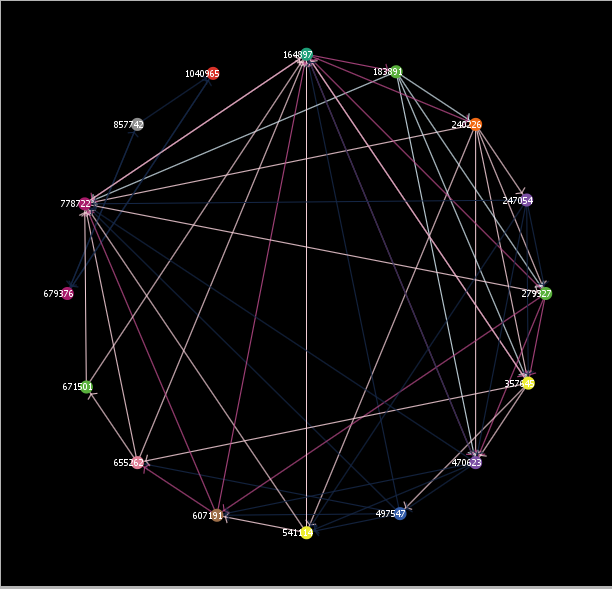
\includegraphics[width=\linewidth]{example_problem}
\caption{ADD CAPTION}
\label{problem}
\end{figure}


\begin{figure}
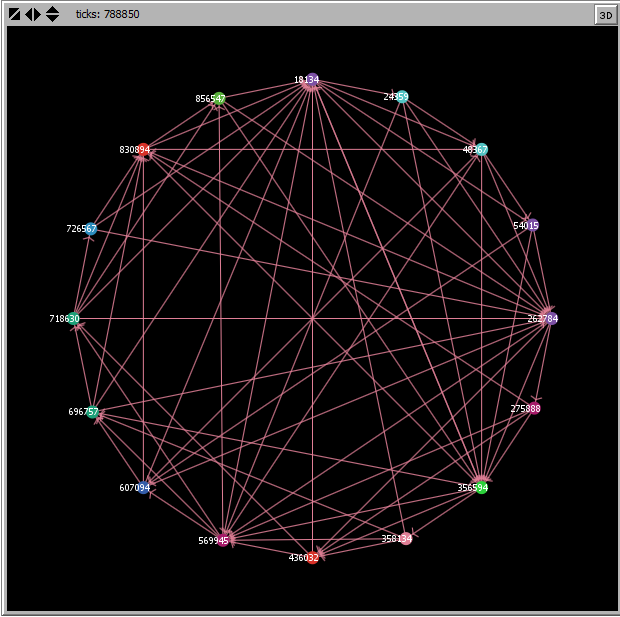
\includegraphics[width=\linewidth]{fixed_example}
\caption{MOAR CAPTION}
\label{fixed}
\end{figure}






\bibliographystyle{plain}
\bibliography{IRMLP}


\end{document}